Consider now the case in which, as in step 3, the conversion rates are unknown but also the values of the graph weights.\\ These parameters gave us the probability that a customer clicks on the secondary product having a given product as primary.\\ Therefore, we initialize both learners (UCB-1 and TS) with the graph weights all set to 1.\\ 
In the same way as the previous step, below is reported only the additional calculus to estimate the new unknown parameters.

\subsection{UCB-1}
As said before the first five steps are the same, so here is reported how the graph weights are estimated:
\begin{equation}
    estimated\_graph[p,:] = \frac{estimated\_graph[p,:] * bought[p] + clicks[p,:]}{tot\_bought[p]}
\end{equation}Where: \begin{itemize}
    \item estimated\_graph[p,:] is the vector of all the weights of the graph that starts from the node with the product {\bf p}
    \item bought[p] is the number of times the product {\bf p} has been bought until the day before
    \item clicks[p,:] is the row of the matrix that reports the number of times an edge of the graph has been activated, which means that a click on the secondary product (columns) has been recorded given a primary product (row). So here we look at all the edge that has been activated starting by the primary product {\bf p}
    \item tot\_bought[p] is the number of times the product {\bf p} has been bought until today (so it is bought[p] plus the number of times product p has been bought today)
\end{itemize}
\subsection{TS}
In this case, the Thomson Sampling does exactly the same as the UCB-1 to estimate the graph weights.
\newpage
\subsection{Results}
Also in this case the results are very similar to the previous step: both algorithms perform a little bit worse than in the case in which only one parameter was uncertain (conversion rates).\\ Another thing that remains unchanged is that TS performed better than UCB-1 by reaching the optimal super arm faster.
\begin{multicols}{2}
    \begin{figure}[H]
        \begin{center}
        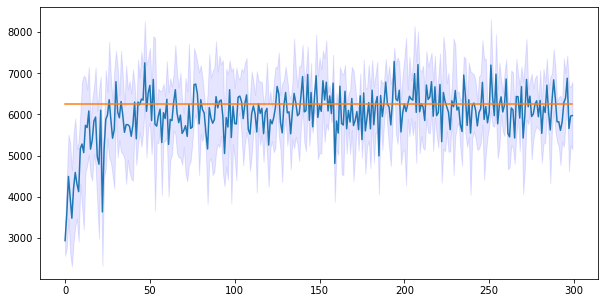
\includegraphics[width=0.5\textwidth]{img/ucb_reward5.png}
        \caption{UCB Reward}
        \label{fig:reward51}
        \end{center}
    \end{figure}
    \columnbreak
    \begin{figure}[H]
        \begin{center}
        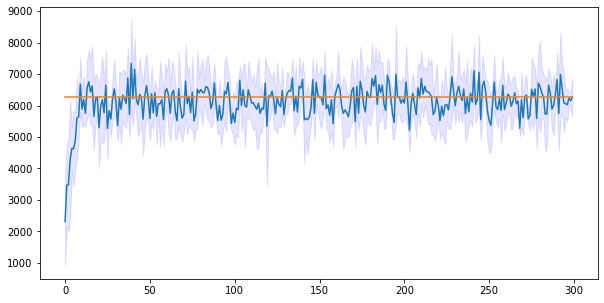
\includegraphics[width=0.5\textwidth]{img/ts_reward5.png}
        \caption{TS Reward}
        \label{fig:reward52}
        \end{center}
    \end{figure}
\end{multicols}

\begin{multicols}{2}
    \begin{figure}[H]
        \begin{center}
        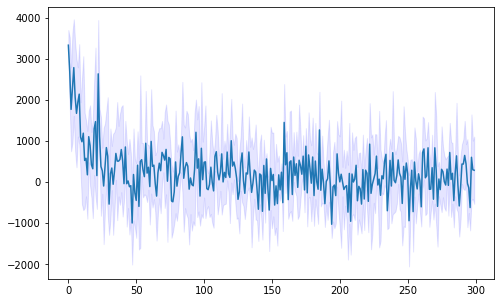
\includegraphics[width=0.5\textwidth]{img/ucb_regret5.png}
        \caption{UCB Regret}
        \label{fig:regret51}
        \end{center}
    \end{figure}
    \columnbreak
    \begin{figure}[H]
        \begin{center}
        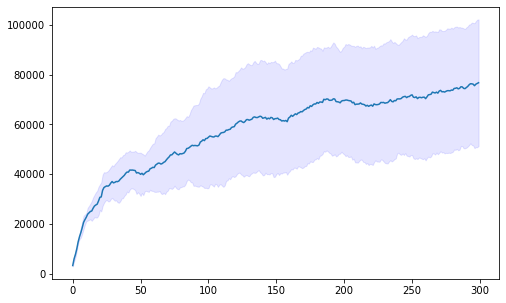
\includegraphics[width=0.5\textwidth]{img/ucb_cum_regret5.png}
        \caption{UCB Cumulative regret}
        \label{fig:cum_reg51}
        \end{center}
    \end{figure}
\end{multicols}
\begin{multicols}{2}
    \begin{figure}[H]
        \begin{center}
        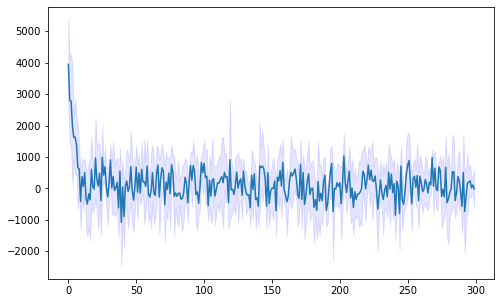
\includegraphics[width=0.5\textwidth]{img/ts_regret5.png}
        \caption{TS Regret}
        \label{fig:regret52}
        \end{center}
    \end{figure}
    \columnbreak
    \begin{figure}[H]
        \begin{center}
        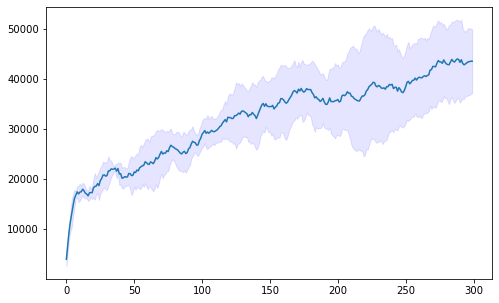
\includegraphics[width=0.5\textwidth]{img/ts_cum_regret5.png}
        \caption{TS Cumulative regret}
        \label{fig:cum_reg52}
        \end{center}
    \end{figure}
\end{multicols}
